\begin{center}
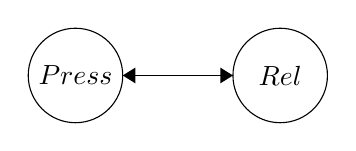
\begin{tikzpicture}[scale=0.2]
\tikzstyle{every node}+=[inner sep=0pt]
\draw [black] (34.9,-27.1) circle (3);
\draw (34.9,-27.1) node {$Rel$};
\draw [black] (21.9,-27.1) circle (3);
\draw (21.9,-27.1) node {$Press$};
\draw [black] (31.9,-27.1) -- (24.9,-27.1);
\fill [black] (24.9,-27.1) -- (25.7,-27.6) -- (25.7,-26.6);
\draw [black] (24.9,-27.1) -- (31.9,-27.1);
\fill [black] (31.9,-27.1) -- (31.1,-26.6) -- (31.1,-27.6);
\end{tikzpicture}
\end{center}